\begin{figure}
    \centering
    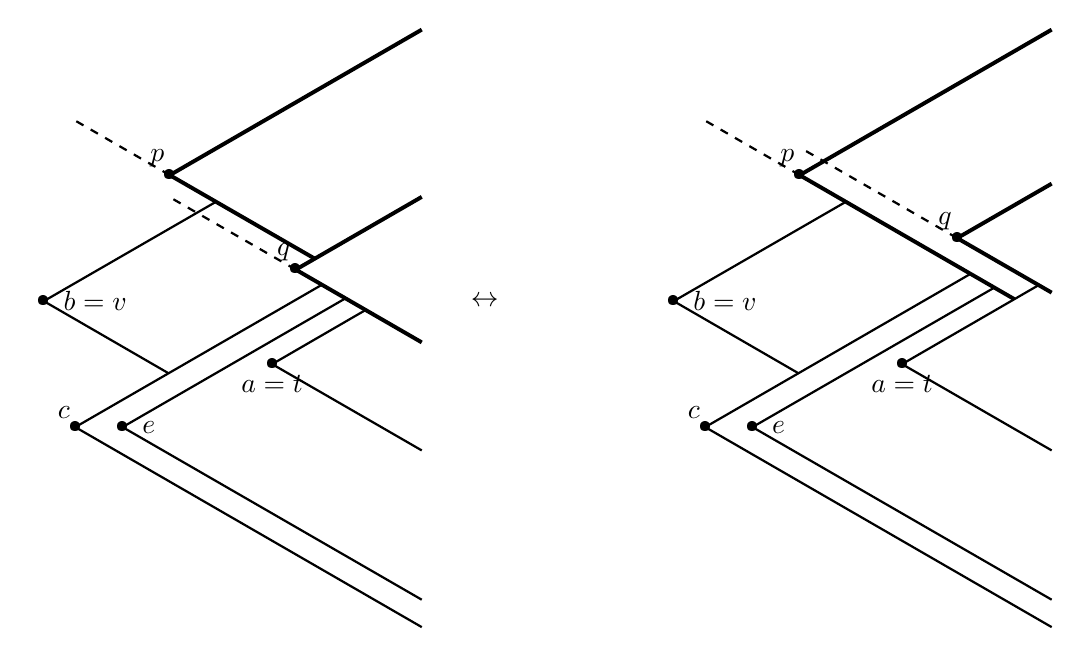
\begin{tikzpicture}[thick, scale=0.4]
        \node[label={[label distance = -3mm]160:$p$}] at
        (2.00, 4.00) {\textbullet};
        \node[label={[label distance = -3mm]160:$q$}] at
        (6.00, 1.00) {\textbullet};
        \node[label={[label distance = -2mm]270:$a = t$}] at
        (5.25, -2.00) {\textbullet};
        % \node[label={[label distance = -3mm]160:$b$}] at (-5.00, 0.00) {\textbullet};
        \node[label={[label distance = -3mm]160:$c$}] at
        (-1.00, -4.00) {\textbullet};
        \node[label={[label distance = -1mm]0:$b = v$}] at
        (-2.00, 0.00) {\textbullet};
        \node[label={[label distance = -1mm]0:$e$}] at
        (0.50, -4.00) {\textbullet};

        % q cone
        \draw[line width = 0.5mm] (6.00, 1.00) -- (10.00, -1.31);
        \draw[line width = 0.5mm] (6.00, 1.00) -- (10.00, 3.31);
        % a cone
        \draw (5.25, -2.00) -- (10.00, -4.74);
        \draw (5.25, -2.00) -- (8.22, -0.28);
        % p cone
        \draw[line width = 0.5mm] (2.00, 4.00) -- (6.60, 1.35);
        \draw[line width = 0.5mm] (2.00, 4.00) -- (10.00, 8.62);
        % c cone
        \draw (-1.00, -4.00) -- (10.00, -10.35);
        \draw (-1.00, -4.00) -- (6.83, 0.52);
        % e cone
        \draw (0.50, -4.00) -- (10.00, -9.48);
        \draw (0.50, -4.00) -- (7.58, 0.09);
        % b cone
        \draw (-2.00, 0.00) -- (1.96, -2.29);
        \draw (-2.00, 0.00) -- (3.46, 3.15);
        % b cone
        % \draw (-5.00, 0.00) -- (0.46, -3.15);
        % \draw (-5.00, 0.00) -- (10.00, 8.66);

        \draw[dashed] (2.00, 4.00) -- (-1.00, 5.73);
        \draw[dashed] (6.00, 1.00) -- (2.00, 3.30);
        \node at (12, 0) {$ \leftrightarrow$};

        \node[label={[label distance = -3mm]160:$p$}] at
        (22.00, 4.00) {\textbullet};
        \node[label={[label distance = -3mm]160:$q$}] at
        (27.00, 2.00) {\textbullet};
        \node[label={[label distance = -2mm]270:$a = t$}] at
        (25.25, -2.00) {\textbullet};
        % \node[label={[label distance = -3mm]160:$b$}] at (15.00, 0.00) {\textbullet};
        \node[label={[label distance = -3mm]160:$c$}] at
        (19.00, -4.00) {\textbullet};
        \node[label={[label distance = -1mm]0:$b = v$}] at
        (18.00, 0.00) {\textbullet};
        \node[label={[label distance = -1mm]0:$e$}] at
        (20.50, -4.00) {\textbullet};

        % q cone
        \draw[line width = 0.5mm] (27.00, 2.00) -- (30.00, 0.27);
        \draw[line width = 0.5mm] (27.00, 2.00) -- (30.00, 3.73);
        % a cone
        \draw (25.25, -2.00) -- (30.00, -4.74);
        \draw (25.25, -2.00) -- (29.59, 0.51);
        % p cone
        \draw[line width = 0.5mm] (22.00, 4.00) -- (28.82, 0.06);
        \draw[line width = 0.5mm] (22.00, 4.00) -- (30.00, 8.62);
        % e cone
        \draw (20.50, -4.00) -- (30.00, -9.48);
        \draw (20.50, -4.00) -- (28.18, 0.43);
        % c cone
        \draw (19.00, -4.00) -- (30.00, -10.35);
        \draw (19.00, -4.00) -- (27.43, 0.87);
        % b cone
        \draw (18.00, 0.00) -- (21.96, -2.29);
        \draw (18.00, 0.00) -- (23.46, 3.15);
        % b cone
        % \draw (15.00, 0.00) -- (20.46, -3.15);
        % \draw (15.00, 0.00) -- (30.00, 8.66);

        \draw[dashed] (22.00, 4.00) -- (19.00, 5.73);
        \draw[dashed] (27.00, 2.00) -- (22.00, 4.88);
    \end{tikzpicture}
    \caption{Da esquerda para a direita, o caso em que $p$ está em
        $\Hits_{low}(q)$, ou seja, $q$ está entrando em $\Dom(p)$. Da direita
        para a esquerda, o caso em que $q$ está em $\Cands(p)$, saindo de
        $\Dom(p)$.}
    \label{fig:parcinetico:eventoup}
\end{figure}